\chapter{Implementation}
\label{Implementation}

% Software & Hardware Requirements
% Code implementation details (brief descriptions, screenshots)
% Features and functionalities

\section{Software Requirements}
\subsection{Operating System Requirements}
Fasttrack requires a modern operating system that supports web browsers and mobile applications. The web platform runs on Windows 7 and above while the mobile app is compatible with Android 7.0 and above. A 64-bit processor with at least 4GB RAM is recommended for smooth performance. The system should support Google Chrome, Firefox, Edge, or Safari for optimal web functionality. 
\subsection{Tools Used}
Various tools that are utilized for the implementation of Fasttrack are:
\subsubsection{HTML}
The FastTrack website uses HTML to structure its content, including login, package management and employee assignment sections. It employs semantic elements like <form>, <table>, <div>, and <button> to enhance accessibility and organization. The login and registration forms use <input> fields for credentials, while <table> elements display package and employee details. Navigation is handled with <nav>, and <header> and <footer> provide structured branding. HTML ensures compatibility across devices and browsers, improving SEO and accessibility. Combined with CSS and JavaScript, it enables dynamic interactions like employee assignment. HTML also integrates seamlessly with Firebase and Flask for backend operations.
\subsubsection{CSS}
The FastTrack web application uses CSS to enhance the visual appeal and responsiveness of its interface. It employs Flexbox and Grid for layout management, ensuring a structured and adaptable design. Custom styling is applied to buttons, tables and forms for a professional look and improved usability. Media queries make the website responsive across different screen sizes, from desktops to mobile devices. Hover effects and animations improve user interaction, making navigation more intuitive. CSS variables and reusable classes ensure consistency across pages. The design follows a clean and modern aesthetic, improving the user experience for companies and employees.
\subsubsection{JavaScript}
The FastTrack website uses JavaScript to add interactivity and dynamic functionality. It handles form validation, ensuring correct user input before submission. AJAX requests enable seamless data fetching from the backend without reloading the page. Event listeners manage user interactions, such as button clicks and form submissions. JavaScript updates the UI dynamically, like displaying assigned packages without refreshing. It integrates with Firebase for real-time updates on package assignments and employee status. Third-party libraries, such as Google Maps API, enhance location-based features. The script ensures a smooth and efficient user experience across the platform.
\subsubsection{Python}
The FastTrack website uses Python for backend development, primarily with Flask. Flask handles HTTP requests and serves data to the frontend via REST APIs. It integrates with Firebase Firestore, managing company, employee and package data efficiently. Python processes uploaded Excel files, extracting package details for assignment. The employee assignment algorithm is implemented in Python, optimizing route efficiency. It also manages authentication and authorization, ensuring secure access to company and admin functionalities. Python’s flexibility and Flask’s lightweight nature enable a scalable and efficient backend for FastTrack.
\subsubsection{Flutter}
The FastTrack mobile app is built using Flutter, a cross-platform framework for developing high-performance applications. Dart is the primary language, enabling smooth UI and efficient state management. The app integrates with Firebase Authentication for secure employee login and Firestore for real-time package updates. Google Maps API is used for location input, navigation, and route optimization, ensuring efficient deliveries. The app supports push notifications via Firebase to keep employees updated. With Flutter's widget-based approach, the app offers a responsive and interactive user experience across Android devices.
\subsubsection{Firebase}
Firebase is essential for the FastTrack system, providing a secure and scalable backend. Firebase Authentication ensures safe logins for companies and employees. Cloud Firestore stores real-time data, including employee details, package assignments and delivery status updates. Firebase Hosting can be used to deploy the web portal efficiently. With Google’s robust infrastructure, Firebase enables seamless data synchronization and real-time updates across devices. It simplifies backend management, eliminating the need for a separate server while ensuring high availability and security.
\subsubsection{Google Maps API}
The Google Maps API is used in the FastTrack to enhance location-based features in the Flutter app. It enables map rendering, real-time GPS tracking, and dynamic routing for delivery personnel. Directions API helps in generating optimized routes for multiple deliveries, ensuring efficient navigation. Geocoding API converts addresses into coordinates for precise location storage. Maps customization allows branding adjustments to align with FastTrack’s theme. With real-time updates and interactive map controls, the API ensures a seamless and intuitive delivery experience.
\subsubsection{Supabase}
Supabase is used for storing images in FastTrack as a scalable and secure alternative to Firebase Cloud Storage. It provides PostgreSQL-backed storage, ensuring efficient retrieval and management of profile and package images. It provides a direct URL link for each uploaded image, making it easy to retrieve and display images in the FastTrack app. These links can be stored in Firestore alongside other user or package data for quick access. 
\section{Hardware Requirements}
\subsection{Website}
\begin{enumerate}
    \item Processor: At least an Intel i3 (or AMD equivalent), but i5/i7 is recommended for smooth multitasking.
    \item RAM: Minimum 4GB, recommended 8GB or higher for handling multiple browser tabs and development tools.
    \item Internet Connection: A stable broadband connection (at least 10 Mbps) for real-time interactions with cloud-based services.
\end{enumerate}
\subsection{Mobile App}
\begin{enumerate}
    \item Processor: A 1.4 GHz or higher multi-core processor to ensure smooth app execution and real-time processing.
    \item RAM: At least 2GB for basic performance, with 4GB or more recommended for handling maps and real-time updates efficiently.
    \item Connectivity: Stable 4G/5G, GPS and Wi-Fi support for seamless real-time data transmission and location tracking.
\end{enumerate}
\section{Code Implementation Details}
\subsection{Authentication \& Authorization}
FastTrack uses Firebase Authentication for secure login and access control. Employees and companies authenticate using email and password, while the system verifies credentials and maintains session states. The authentication logic ensures that only authorized users can access package details and employee assignments.
\subsection{Package Assignment}
Package details are uploaded via an Excel file, processed using Python (Flask), and stored in Firestore. Each package entry includes recipient details, location coordinates, and assigned delivery personnel. The system updates package status dynamically based on delivery progress.
\subsection{Employee Assignment}
The system calculates the required number of employees based on the uploaded package data. Companies select available employees and packages are automatically assigned using a assignment algorithm that minimizes travel distance. The assignments are updated in Firestore for real-time access by employees.
\subsection{Route Optimization \& Navigation}
The Google Maps API is integrated into the mobile app to assist delivery personnel. Employees can view optimized routes and track package drop-off points.
Optimized route generation in FastTrack is based on a greedy algorithm, ensuring efficient delivery route planning. The app dynamically updates routes when a delivery is completed.
\subsection{Real-time Updates \& Notifications}
Firestore enables real-time synchronization of package assignments and status updates across the system. Employees receive push notifications (Firebase) for new assignments and delivery updates.
\subsection{Screenshots}
\begin{figure}[H]
\centering
\begin{minipage}{0.6\textwidth}
    \centering
    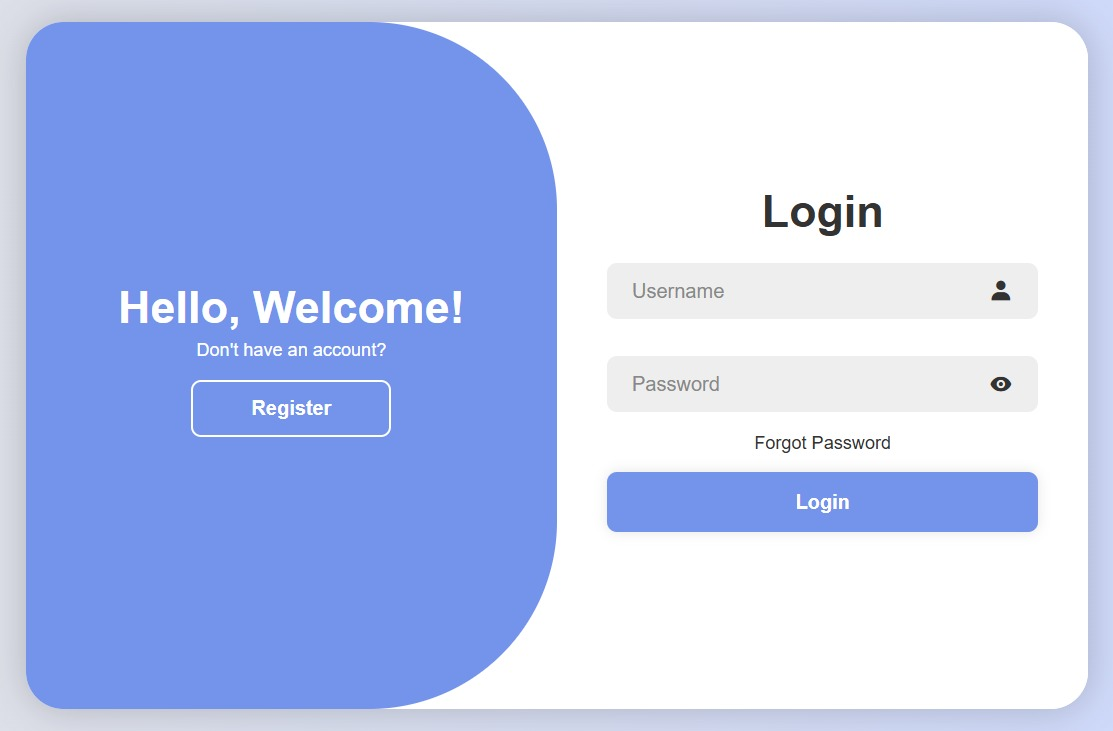
\includegraphics[width=\linewidth]{4/Website_Login.jpg}
    \label{fig:authentication1}
\end{minipage}%
\hspace{5mm}
\begin{minipage}{0.3\textwidth}
    \centering
    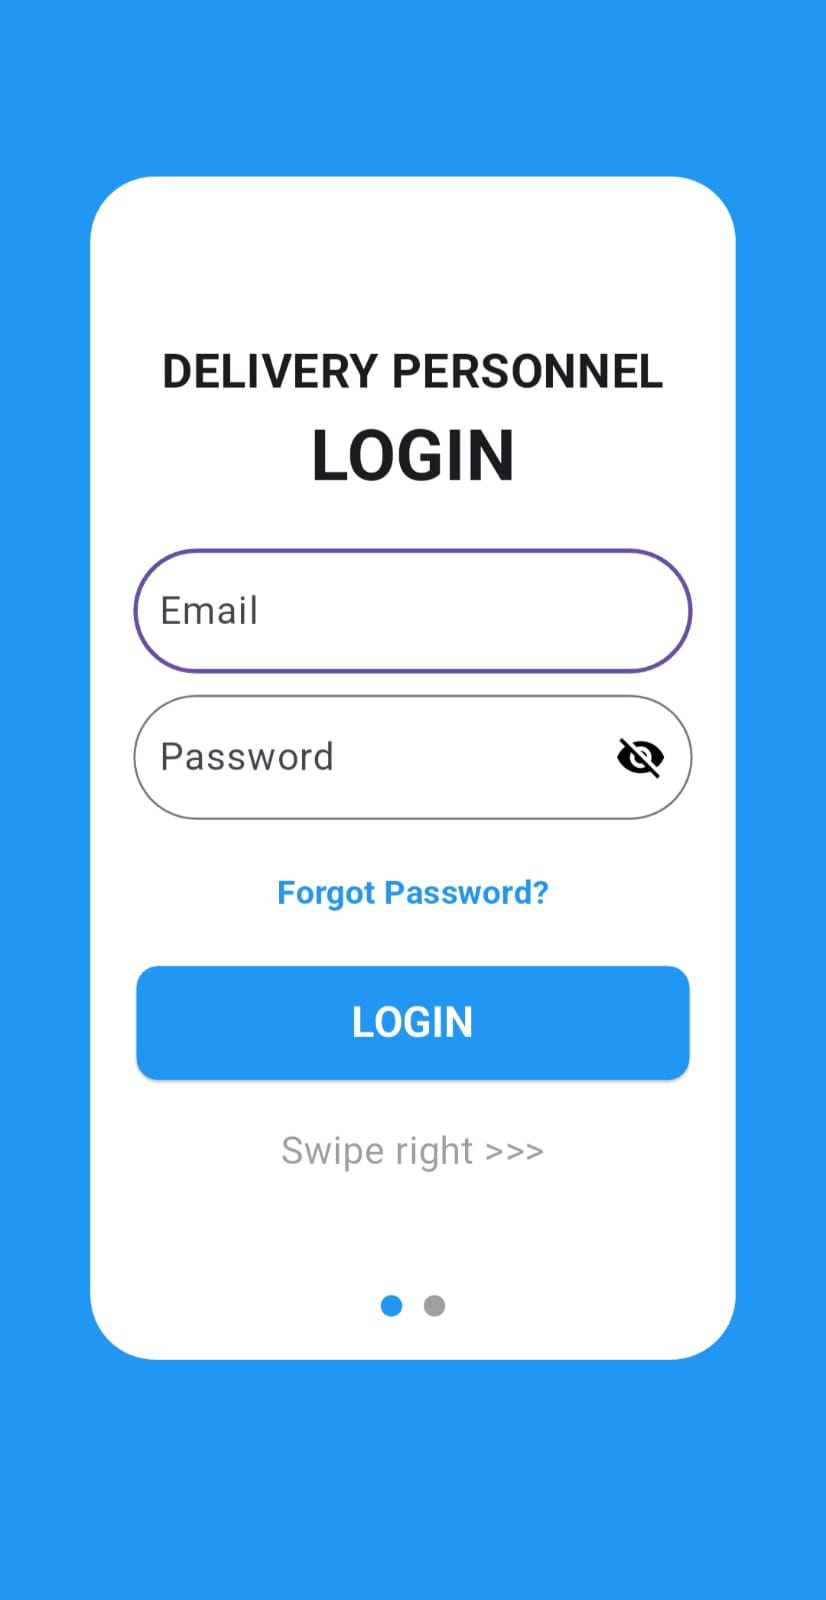
\includegraphics[width=\linewidth]{4/Mobile_login.jpg}
    \label{fig:authentication2}
\end{minipage}
\caption{Authentication \& Authorization}
\label{fig:authentication_combined}
\end{figure}
\begin{figure}[H]  % Use [H] to force the position
\centering
    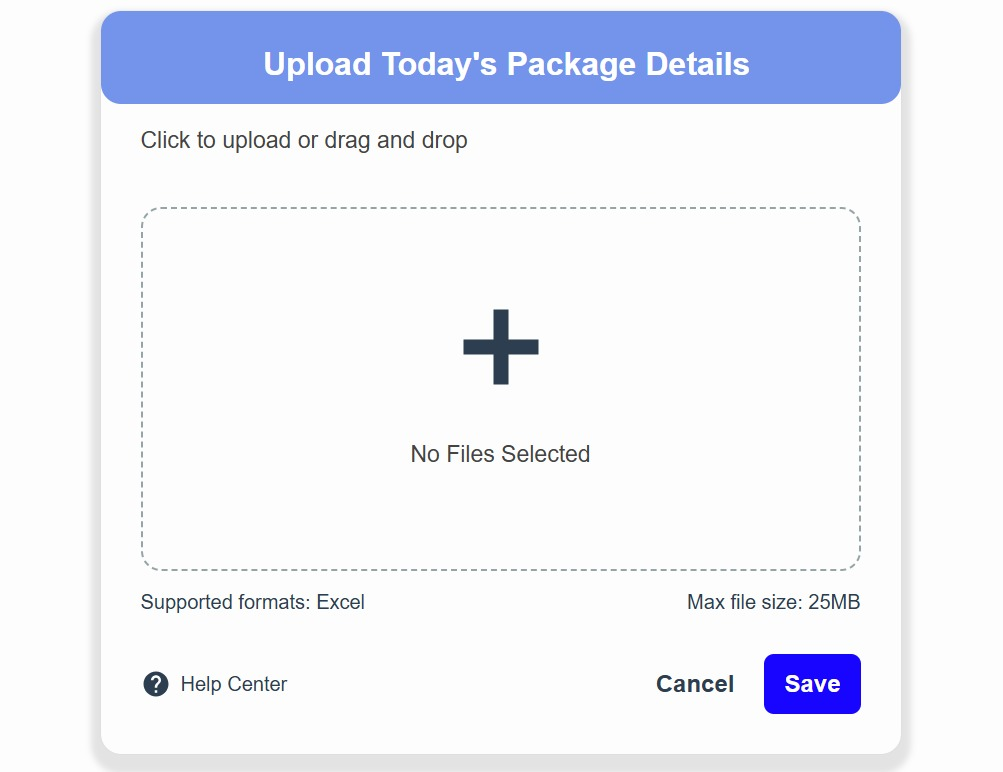
\includegraphics[scale=0.3]{4/Package_Upload.jpg}
    \caption{Package Assignment}
    \label{fig:package_upload}
\end{figure}
\begin{figure}[H]  % Use [H] to force the position
\centering
    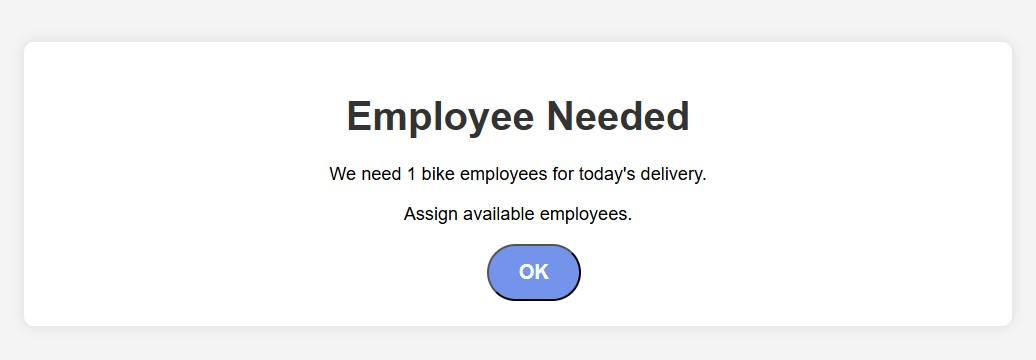
\includegraphics[scale=0.5]{4/Employee1.jpg}
    \caption{Employee Assignment}
    \label{fig:employye_assignment}
\end{figure}
\begin{figure}[H]
\centering
\begin{minipage}{0.24\textwidth}
    \centering
    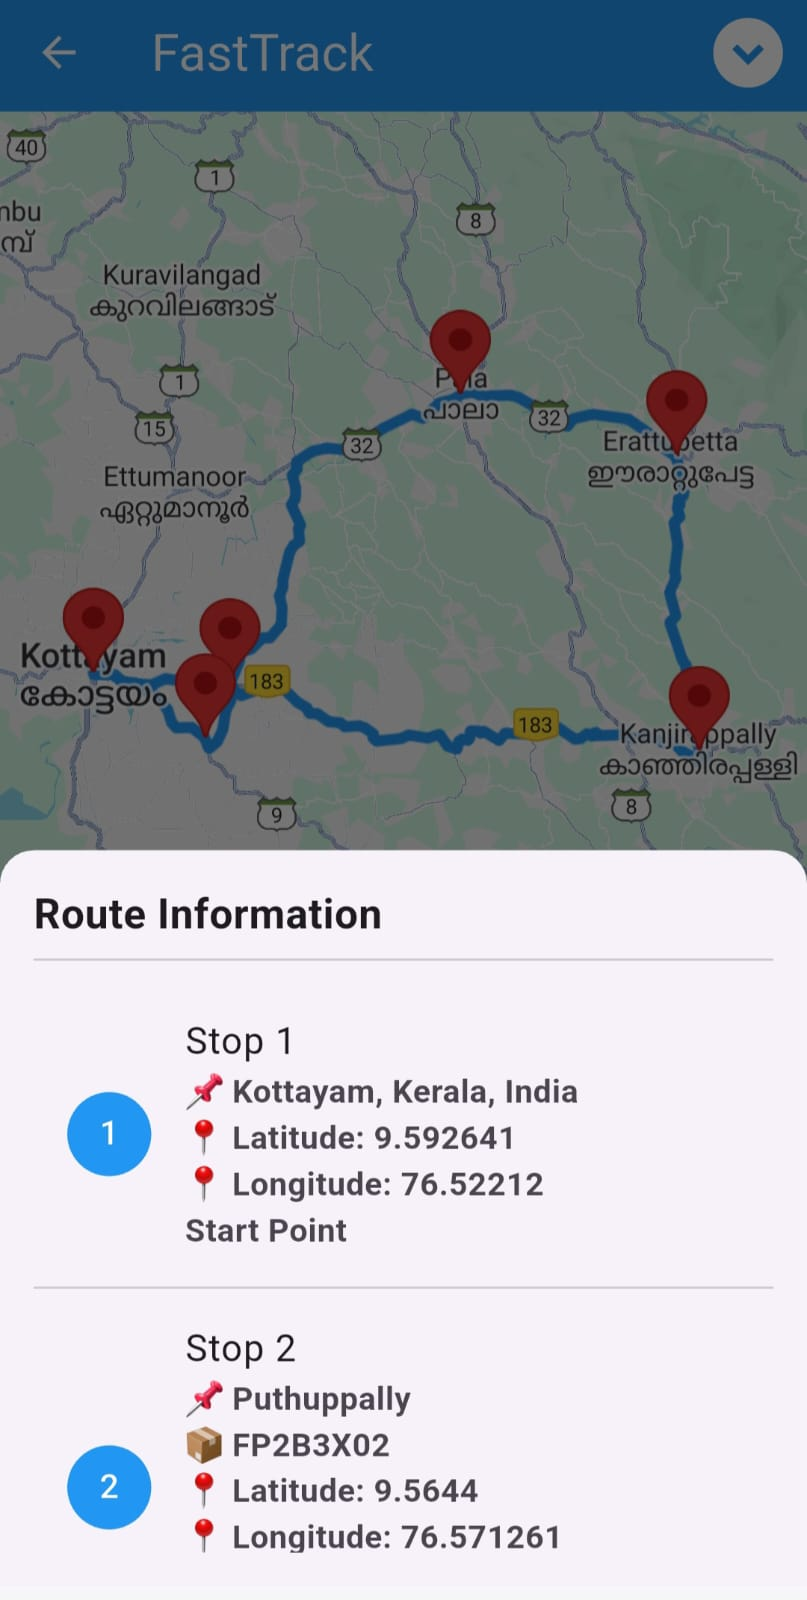
\includegraphics[width=\linewidth]{4/Route_Optimization2.jpg}
    \label{fig:route_optimization2}
\end{minipage}%
\hspace{5mm}
\begin{minipage}{0.24\textwidth}
    \centering
    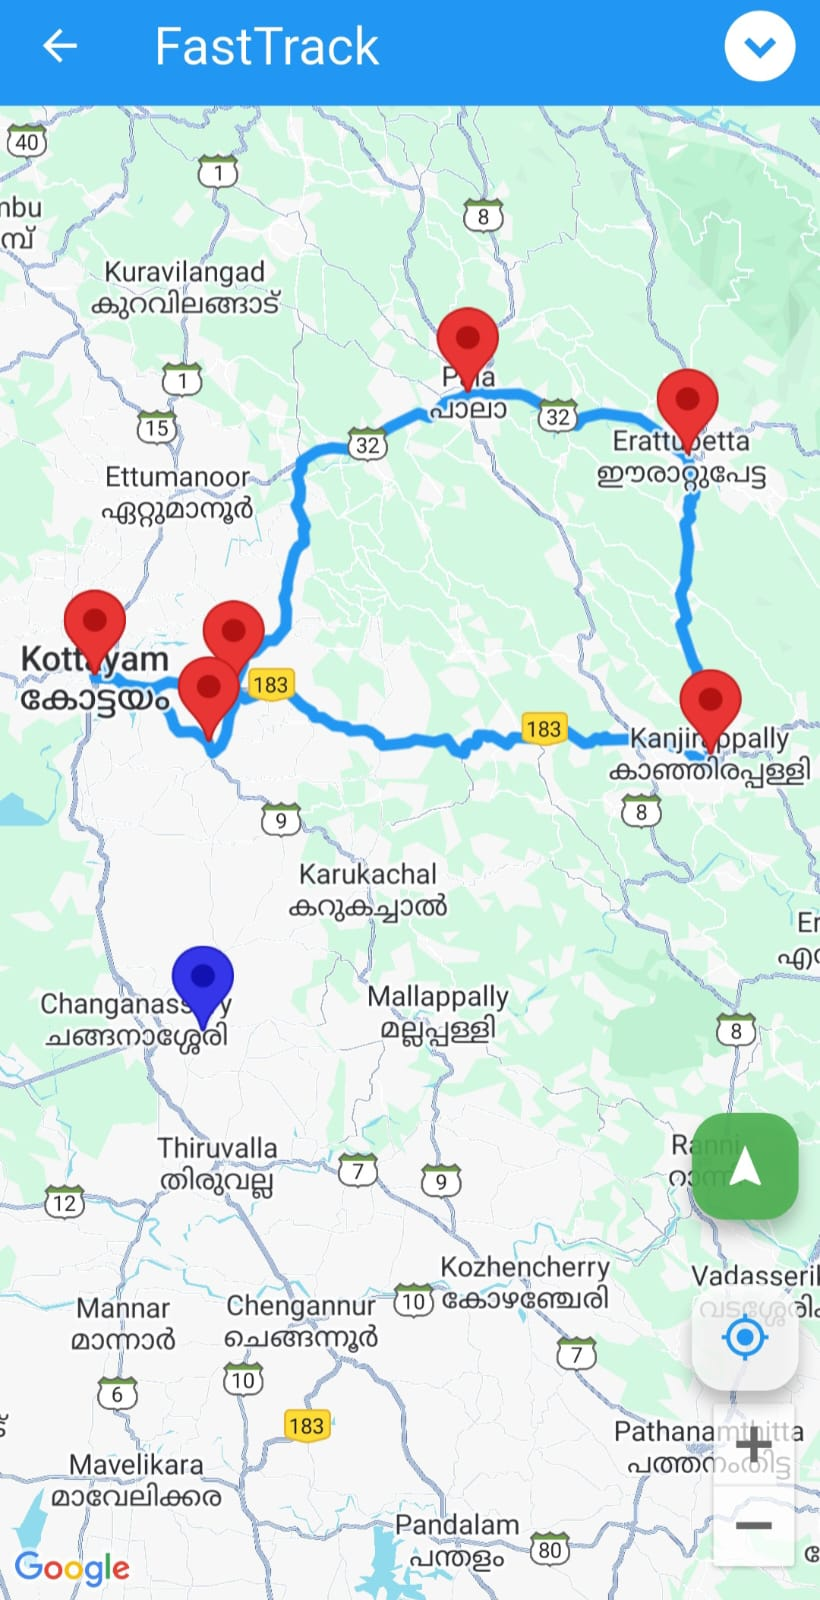
\includegraphics[width=\linewidth]{4/Route_Optimization1.jpg}
    \label{fig:route_optimization1}
\end{minipage}
\caption{Route Optimization and Navigation}
\label{fig:route_optimization_combined}
\end{figure}
\begin{figure}[H]
    \centering
    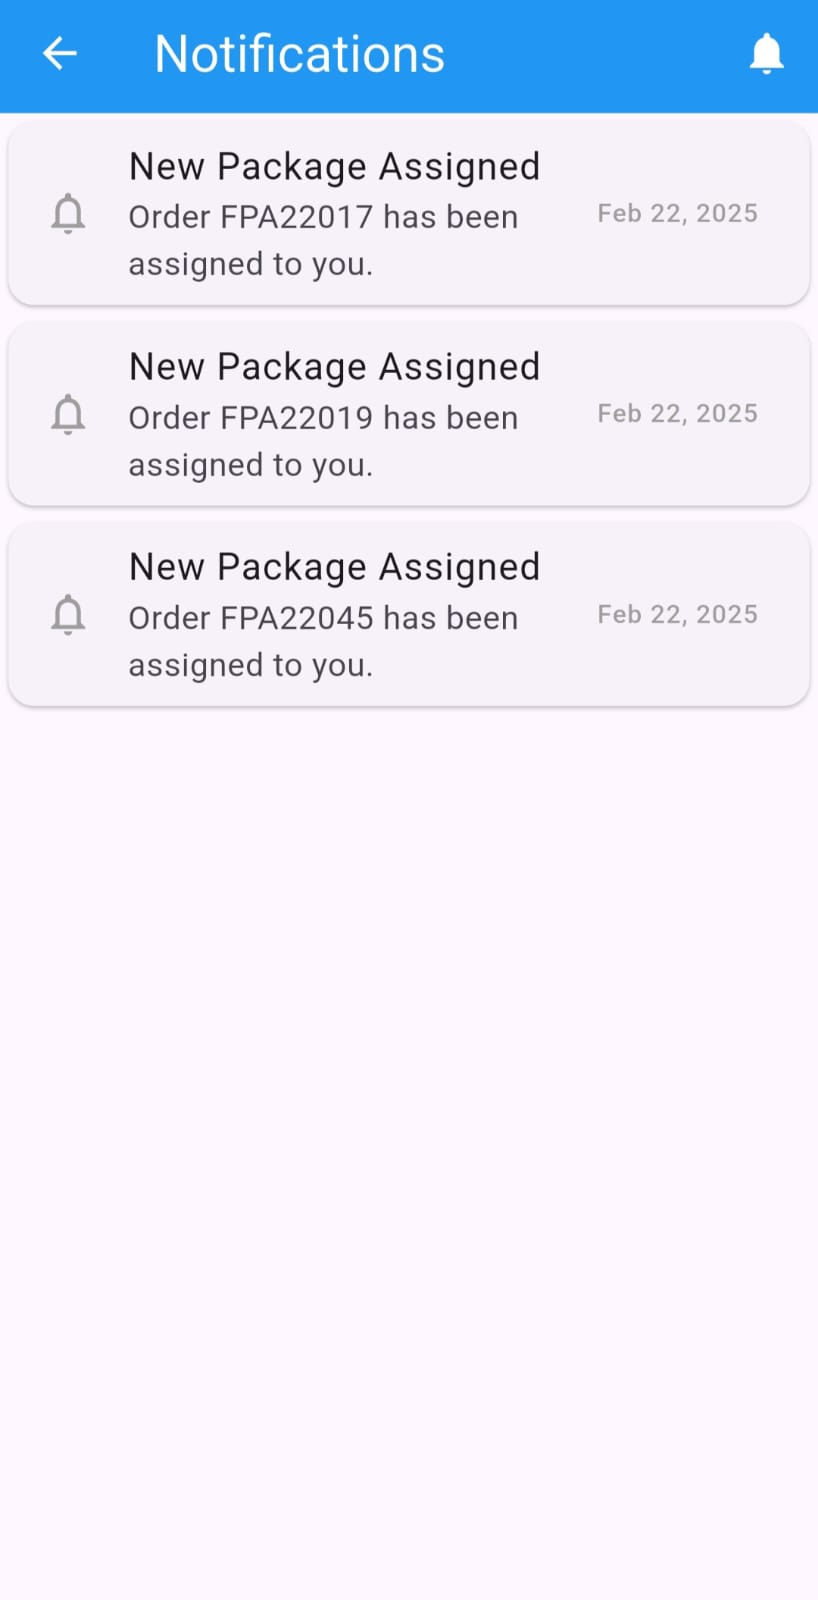
\includegraphics[width=0.24\linewidth]{4/Notification.jpg}
    \caption{Notifications}
    \label{fig:notificationl}
\end{figure}
\newpage
\section{Features and Functionalities}
\subsection{User Authentication \& Management}
\begin{itemize}
    \item Companies can register with required details.
    \item They can login securely using Firebase Authentication.
    \item Companies can add, edit and manage delivery personnel.
    \item Each company gets a unique 5-character alphanumeric ID (FCXXX).
    \item Each employee gets a unique 8-character alphanumeric ID (FDXXXYYY), where XXX wil be Company ID.
    \item Each packet will gets a unique 8-character alphanumeric ID (FPXXXYYY), where XXX wil be Company ID.
\end{itemize}
\subsection{Package Handling \& Assignment}
\begin{itemize}
    \item Companies upload daily package details via an Excel file.
    \item The system calculates the required number of employees based on packages.
    \item Companies assign packages to available delivery personnel.
\end{itemize}
\subsection{QR Code System}
\begin{itemize}
    \item Companies can generate QR codes for each package.
    \item Delivery Personnel can  scan QR codes for picking their assigned package.
\end{itemize}
\subsection{Route Optimization}
\begin{itemize}
    \item Displays the efficient path from the employee’s current location to each delivery stop.
    \item Updates dynamically as deliveries are completed.
\end{itemize}
\section{Summary}
Chapter 4 details the implementation of the FastTrack system, focusing on the technologies and
methodologies used. The section begins with the software and hardware requirements, outlining the
necessary operating systems, devices, and tools such as HTML, CSS, JavaScript, Python (Flask),
Flutter, Firebase and Google Maps API.
It then explains the core functionalities, including user authentication, package handling, QR code
integration and real-time updates. The route optimization module ensures efficient deliveries using
Google Maps API, dynamically updating paths. The backend, built with Firebase and Flask,
manages data storage, user authentication and real-time synchronization.
Finally, the chapter includes the screenshots of implemented code providing a visual representation
. Overall, it provides a comprehensive view of the FastTrack system’s implementation, highlighting
key technologies and workflow.